\documentclass[a4paper]{sbgames}               % final
%\usepackage[scaled=.92]{helvet}
\usepackage{times}
\usepackage{graphicx}

%% use this for zero \parindent and non-zero \parskip, intelligently.
\usepackage{parskip}

%% the 'caption' package provides a nicer-looking replacement
\usepackage[labelfont=bf,textfont=it]{caption}

\usepackage{url}

\usepackage[latin1]{inputenc}
\usepackage{algorithmic}
\usepackage{algorithm}


\newcommand{\misccite}[2]{#1. Dispon�vel em: \textless#2\textgreater. Acesso em: 26 jun. 2009}
\newcommand{\gamecite}[2]{\misccite{#1}{#2}}

%% Paper title.
\title{Utilizando kd-trees para particionar o ambiente virtual e balancear dinamicamente a carga sobre servidores de MMOGs}

%% Author and Affiliation (multiple authors). Use: and between authors

\author{Carlos Eduardo B. Bezerra, Jo�o L. D. Comba, Cl�udio F. R. Geyer\\
				Instituto de Inform�tica\\
				Universidade Federal do Rio Grande do Sul\\
				Av. Bento Gon�alves, 9500, Porto Alegre
}
\contactinfo{\{carlos.bezera, comba, geyer\}@inf.ufrgs.br
}
%% Keywords that describe your work.
\keywords{MMOGs, load balancing, distributed server, kd-trees.}

%% Start of the paper
% Attention: As you need to insert EPS images in Postscript, 
% you need to insert PDF images into PDFs. 
% In the text, extensions cancbe omitted (latex use .eps, pdflatex get .pdf) 
% To convert them: epstopdf myimage.eps
\begin{document}

%\teaser{
%  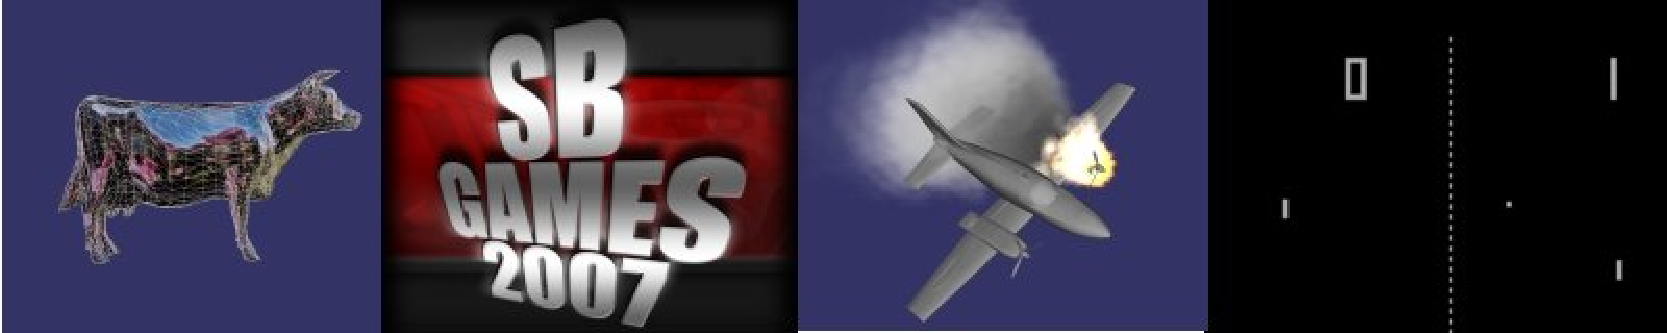
\includegraphics[width=\linewidth]{sample.pdf}
%  \caption{Optional image}
%}

%% The ``\maketitle'' command must be the first command after the
%% ``\begin{document}'' command. It prepares and prints the title block.

\maketitle

%% Abstract section.

\begin{abstract}
MMOGs (massively multiplayer online games) are applications that require high bandwidth connections to work properly. This demand for bandwidth is specially critical on the servers that host the game. This happens because the typical number of simultaneous participants in this kind of game varies from a few hundreds to several tens of thousands, and the server is the one responsible for mediating the interaction between every pair of players connected to it. To deal with this problem, decentralized architectures with multiple servers have been proposed, where each server manages a region of the virtual environment of the game. Each player, then, connects only to the server that manages the region where he is playing. However, to distribute the load among the servers, it is necessary to devise an algorithm for partitioning the virtual environment. In order to readjust the load distribution during the game, this algorithm must be dynamic. Some work has already been made in this direction, but using a geometric algorithm, more appropriate than those found in the literature, it should be possible to reduce the distribution granularity without compromising the rebalancing time, or even reducing it. In this work, we propose the use of a kd-tree for dividing the virtual environment of the game in regions, each of which being designated to one of the servers. The split coordinates of the regions are adjusted dynamically according to the distribution of avatars in the virtual environment. We compared our algorithm to some approaches found in the literature and the simulation results show that our algorithm performed better in most aspects we analysed.
\end{abstract}

%% The ``\keywordlist'' command prints out the keywords.
\keywordlist
\contactlist

\section{Introduction}

The main characteristic of MMOGs is the large number of players interacting simultaneously, reaching the number of tens of thousands \cite{schiele2007rpp}. When using a client-server architecture for the players to communicate with one another, the server intermediates the communication between each pair of players.

To allow the interaction of players, each one of them sends his commands to the server, which calculates the resulting game state and sends it to all the players to whom the state change is relevant. We can see that the number of state update messages sent by the server may grow proportionally to the square of the number of players, if all players are interacting with one another. Obviously, depending on the number of players, the cost of maintaining a centralized infrastructure like this is too high, restricting the MMOG market to large companies with enough resources to pay the upkeep of the server.

In order to reduce this cost, several decentralized solutions have been proposed. Some of them use peer-to-peer networks, such as \cite{schiele2007rpp,rieche2007ppb,hampel2006ppa,elrhalibi2005abm,iimura2004zfg,knutsson2004pps}. Others propose the use of a distributed server composed of low-cost nodes connected through the Internet, as in \cite{ng2002msa,chertov:olb,lee2003sdl,assiotis2006dam}. Anyway, in all these approaches, the ``world'', or virtual environment of the game is divided into regions and for each region is assigned a server -- or a group of peers to manage it, when using peer-to-peer networks. Each of these regions must have a content such that the load imposed on the corresponding server is not greater than its capacity.

When an \emph{avatar} (representation of the player in the virtual environment) is located in a region, the player controlling that avatar connects to the server associated to that region. That server, then, is responsible for receiving the input from that player and for sending, in response, the update messages. When a server becomes overloaded due to an excessive number of avatars in its region and, therefore, more players to be updated, the division of the virtual environment must be recalculated in order to alleviate the overloaded server.

Usually, the virtual environment is divided into relatively small cells, which are then grouped into regions and distributed among the servers. However, this approach has a severe limitation in its granularity, since the cells have fixed size and position. Using a more appropriate geometric algorithm, it should be possible to achieve a better player distribution among different servers, making use of traditional techniques that are generally used for computer graphics.

In this work, we propose the utilization of a kd-tree to perform the partitioning of the virtual environment. When a server is overloaded, it triggers the load balancing, readjusting the limits of its region by changing the split coordinates stored in the kd-tree. A prototype has been developed and used in simulations. The results found in these simulations have been compared to previous results from approaches which use the cell division technique.

The text is organized as follows: in section \ref{context}, some related works are described; in section \ref{sec:proposal}, the algorithm proposed here is presented in detail; in the sections \ref{sec:simul} and \ref{sec:result}, we present, respectively, the simulation details and its results and, in section \ref{sec:conc}, the conclusions of this work are presented.




\section{Related Work}
\label{context}

Different authors have attacked the problem of partitioning the virtual environment in MMOGs for distribution among multiple servers \cite{ahmed2008mol,bezerra2009lbs}. Generally, there is a static division into cells of fixed size and position. The cells are then grouped into regions (Figure \ref{fig:cells}), and each region is delegated to one of the servers. When one of them is overwhelmed, it seeks other servers, which can absorb part of the load. This is done by distributing one or more cells of the overloaded server to other servers.

\begin{figure}[!t]
	\centering
	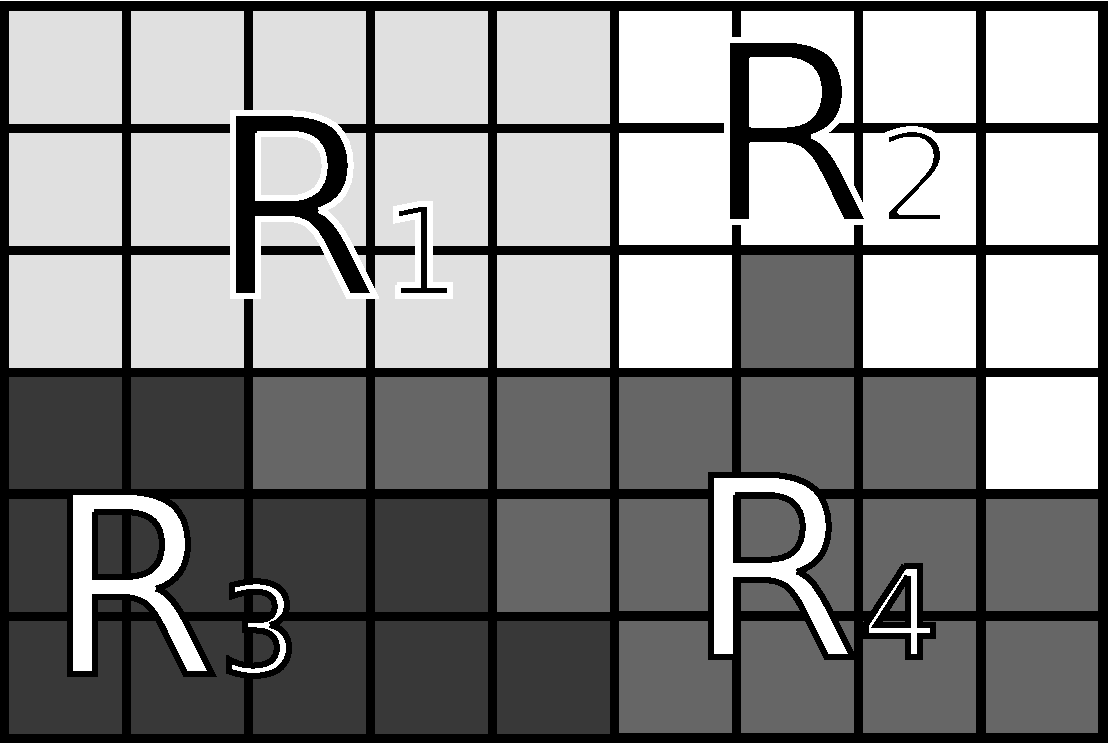
\includegraphics[width=0.85\linewidth]{images/macromicro}
	\caption{Division into cells and grouping into regions}
	\label{fig:cells}
\end{figure}

\cite{ahmed2008mol}, for example, propose a cell-oriented load balancing model. To balance the load, their algorithm finds, first, all clusters of cells that are managed by the overloaded server. The smallest cluster is selected and, from this cluster, it is chosen the cell which has the least interaction with other cells of the same server -- the interaction between two cells A and B is defined by the authors as the number of pairs of avatars interacting with each other, one of them in A and the other one in B. The selected cell is then transferred to the least loaded server, considering ``load'' as the bandwidth used to send send state updates to the players whose avatars are positioned in the cells managed by that server. This process is repeated until the server is no longer overloaded or there is no more servers capable of absorbing more load -- in this case, one option could be to reduce the frequency at which state update messages are sent to the players, as suggested by \cite{bezerra2008a3}.

\begin{figure}[!t]
	\centering
	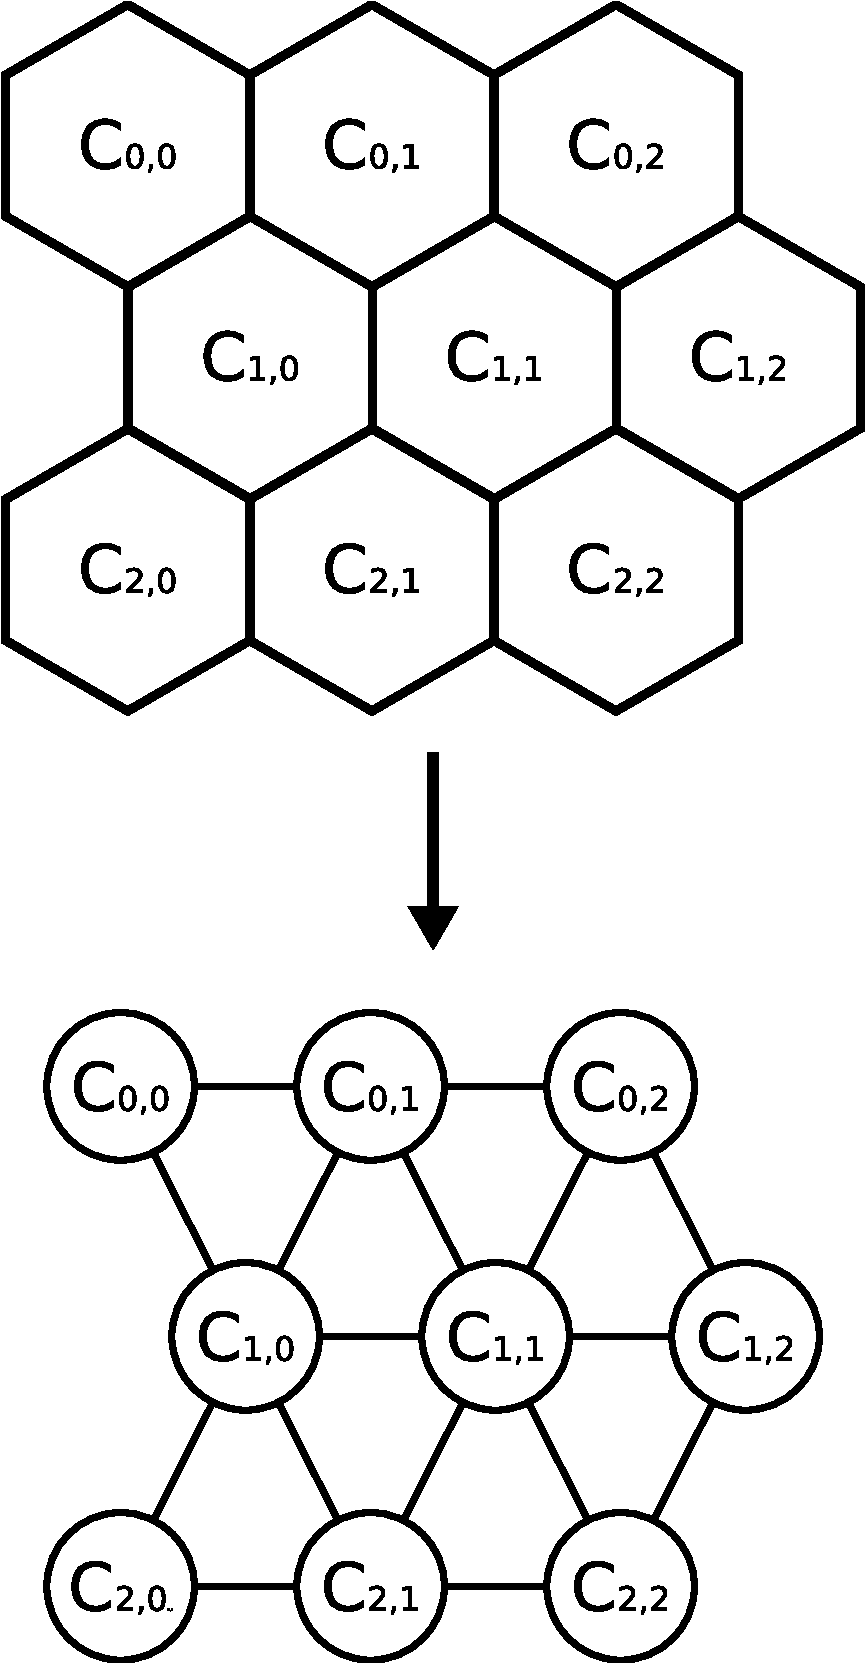
\includegraphics[width=0.5\linewidth]{images/grafo}
	\caption{Graph representation of the virtual environment}
	\label{fig:graph}
\end{figure}

In \cite{bezerra2009lbs}, it is also proposed the division into cells. To perform the division, the environment is represented by a graph (Figure \ref{fig:graph}), where each vertex represents a cell. Each edge in the graph connects two vertices representing neighboring cells. The weight of a vertex is the server's bandwidth occupied to send state updates to the players whose avatars are in the cell represented by that vertex. The interaction between any two cells define the weight of the edge connecting the corresponding vertices. To form the regions, the graph is partitioned using a greedy algorithm: starting from the heaviest vertex, at each step it is added the vertex connected by the heaviest edge to any of the vertices already selected, until the total weight of the partition of the graph -- defined as the sum of the vertices' weights -- reaches a certain threshold related to the total capacity of the server that will receive the region represented by that partition of the graph.

Although this approach works, there is a serious limitation on the distribution granularity it can achieve. If a finer granularity is desired, it is necessary to use very small cells, increasing the number of vertices in the graph that represents the virtual environment and, consequently, the time required to perform the balancing. Besides, the control message containing the of cells designated to each server also become larger. Thus, it may be better to use another approach to perform the partitioning of the virtual environment, possiby using a data structure more suitable, such as a kd-tree \cite{bentley1975mbs}.

This kind of data structure is generally used in computer graphics. However, as in MMOGs there is geometric information -- such as the position of each avatar in the environment --, space partitioning trees could be used. Moreover, we cand find in the literature techniques for keeping the partitions defined by the tree with a similar ``load''. In \cite{luque2005bpc}, for example, it is sought to reduce the time needed to calculate the collisions between pairs of objects moving through space. The authors propose the use of a BSP (binary space partitioning) tree to distribute the objects in the scene (Figure \ref{fig:bsp}). Obviously, if each object of one pair is completely inserted in a different partition, they do not collide and there is no need to perform a more complex test for this pair. Assuming an initial division, it is proposed by the authors a dynamic readjustment of the tree as objects move, balancing their distribution on the leaf-nodes of the tree and, therefore, minimizing the time required to perform the collision detection. Some of the ideas proposed by the authors may be used in the context of load balancing between servers in MMOGs.

\begin{figure}[!t]
	\centering
	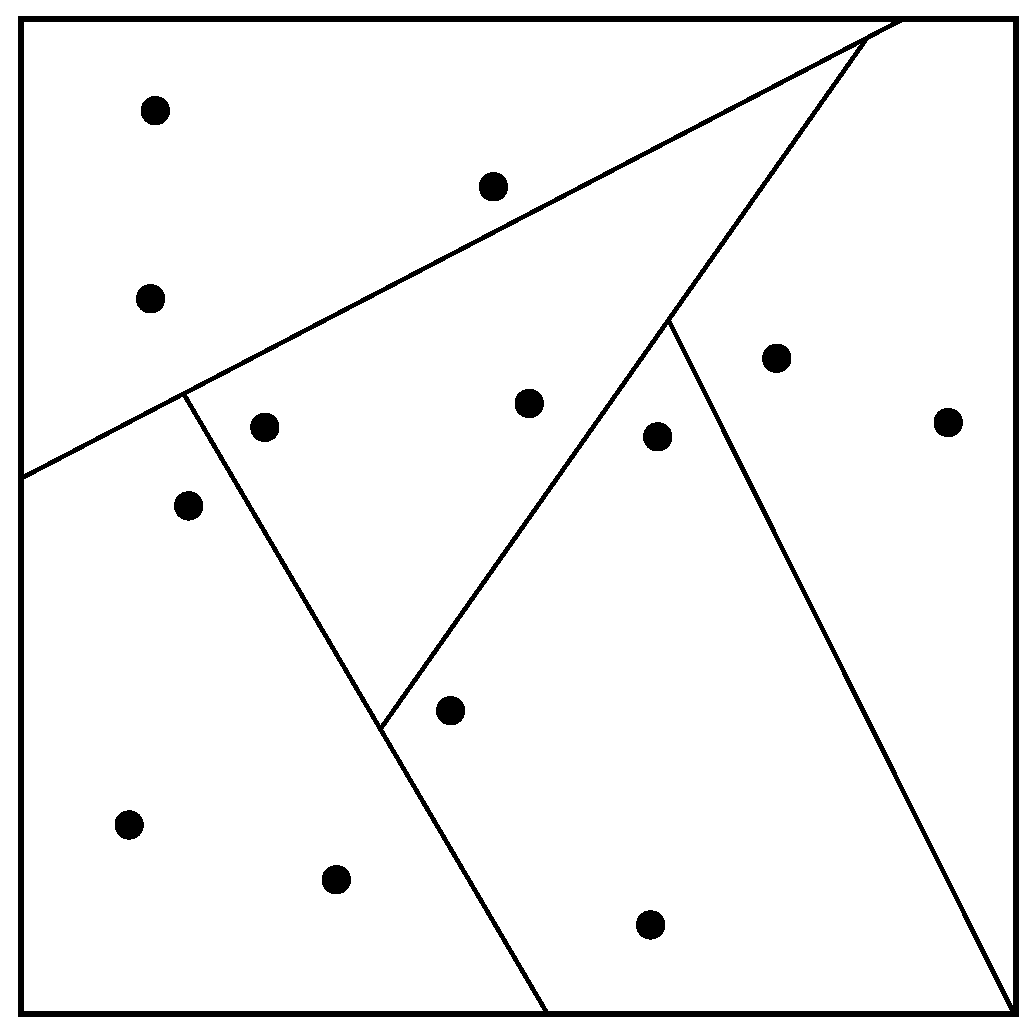
\includegraphics[width=0.5\linewidth]{images/bsp}
	\caption{Space partitioning using a BSP tree}
	\label{fig:bsp}
\end{figure}

\section{FIXME:changetitle Proposed approach}
\label{sec:proposal}

The load balancing approach proposed here is based on two criteria: first, the system should be considere heterogeneous (i.e. each server has a different amount of resources) and, second, the load on each server is \emph{not} proportional to the number of players connected to it, but to the amount of bandwidth required to send state update messages to them.

This choice is due to the fact that each player sends commands to the server at a constant rate, so the number of messages received by the server per unit time grows linearly to the number of players, whereas the number of state update messages sent by the server may be quadratic, in the worst case.

As mentioned in the introduction, to divide the environment of the game into regions, we propose the utilization of a data structure known as kd-tree. The vast majority of MMOGs, such as World of Warcraft \cite{worldofwarcraft}, Ragnarok \cite{ragnarok} and \mbox{Lineage II} \cite{lineage2}, despite having three-dimensional graphics, the simulated world -- cities, forests, swamps and points of interest in general -- in these games is mapped in two dimensions. Therefore, we propose to use a kd-tree with \mbox{k = 2}.

Each node of the tree represents a region of the space and, moreover, in this node it is stored a split coordinate. Each one of the two children of that node represent a subdivision of the region represented by the parent node, and one of them represents the sub-region before the split coordinate and the other one, the sub-region containing points whose coordinates are greter than or equal to the split coordinate. The split axis (in the case of two dimensions, the axis $x$ and $y$) of the coordinate stored alternates for each level of the tree -- if the first level node store x-coordinates, the second level nodes store an y-coordinates and so on. Each leaf node also represents a region of the space, but it does not store any split coordinate. Instead, it stores a list of the avatars present in that region. Finally, each leaf node is associated to a server of the game. When a server is overloaded, it triggers the load balancing, which uses the kd-tree to readjust the split coordinates that define its region, reducing the amount of content managed by it.

Each node of the tree also stores two other values: capacity and load of the subtree. The load of a node is equal to the sum of the load of its children. Similarly, the capacity of a non-leaf node is equal to the sum of the capacity of its children nodes. For the leaf node, these values are the same as the server associated to each one of them. The tree root stores, therefore, the total weight of the game and the total capacity of the server system.

In the following sections, it will be described the construction of the tree, the calculation of the load associated with each server and the proposed balancing algorithm.

\subsection{Building the kd-tree}

To make an initial space division, it is constructed a balanced kd-tree (as far as possible, for it depends on the number of servers -- or leaf nodes -- being equal to a power of 2). For this, we used the recursive function shown in Algorithm \ref{alg:buildtree} to create the tree. cria��o da �rvore.

\begin{algorithm}
\caption{n�::constr�i\_�rvore(id, n�vel, num\_servidores)}
\label{alg:buildtree}
\begin{algorithmic}
	\IF{id + $2^{n\acute{\imath}vel} \ge num\_servidores$ }
		\STATE $filho\_menor \leftarrow filho\_maior \leftarrow NIL$;
		\STATE retorne;
	\ELSE
		\STATE $filho\_menor \leftarrow$ novo\_n�();
		\STATE $filho\_menor.pai \leftarrow$ \textbf{this};
		\STATE $filho\_maior \leftarrow$ novo\_n�();
		\STATE $filho\_maior.pai \leftarrow$ \textbf{this};
		\STATE $filho\_menor$.constr\'oi\_\'arvore\\$(id, n\acute{\imath}vel + 1, num\_servidores)$;
		\STATE $filho\_maior$.constr�i\_\'arvore\\$(id + 2^{n\acute{\imath}vel},$ $n\acute{\imath}vel + 1,$ $num\_servidores)$;
	\ENDIF
\end{algorithmic}
\end{algorithm}

\begin{figure}[!t]
	\centering
	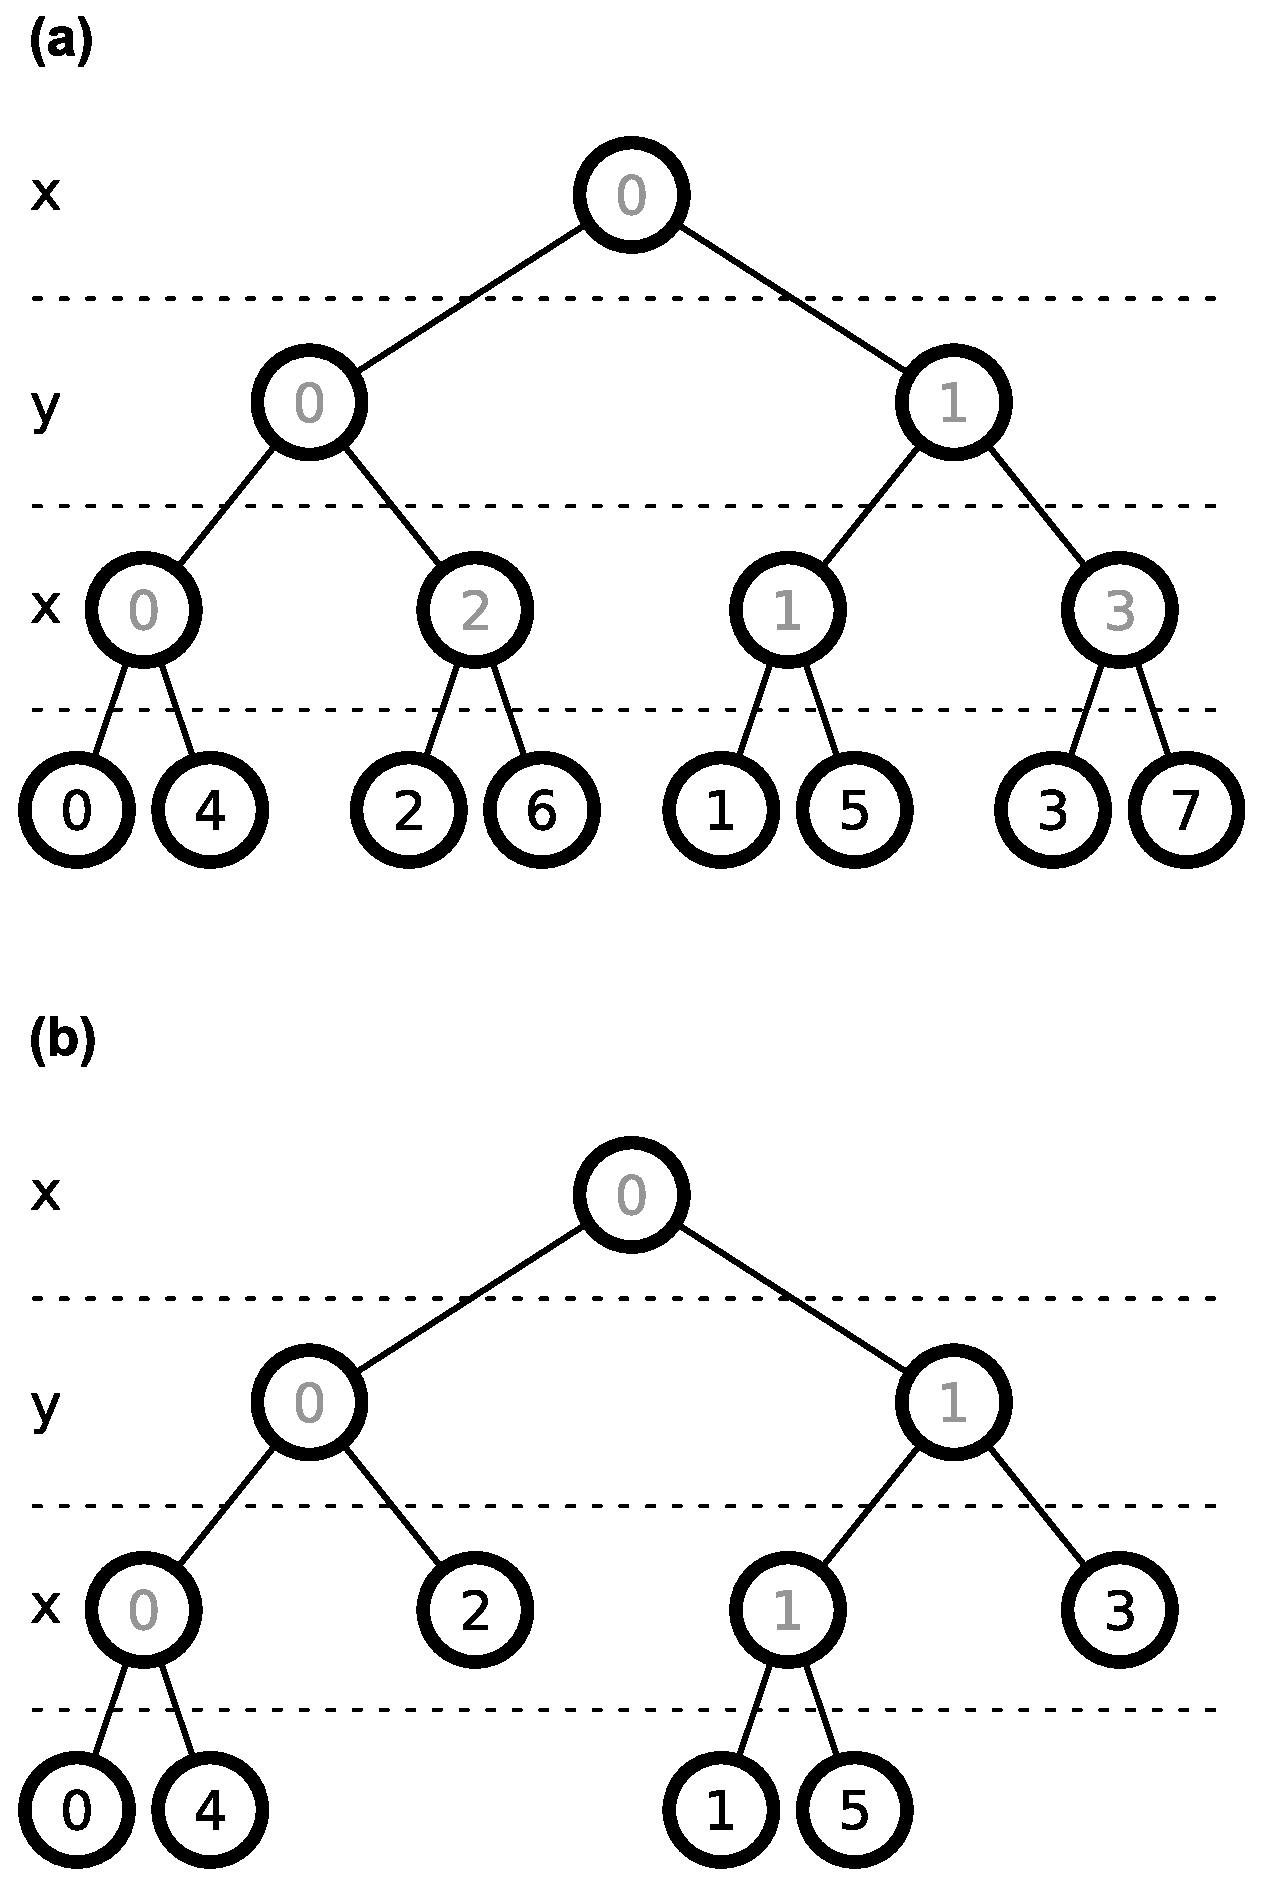
\includegraphics[width=0.75\linewidth]{images/kdtree}
	\caption{Constru��o de kd-tree balanceada}
	\label{fig:kdtree}
\end{figure}

No Algoritmo 1, o $id$ serve para calcular quantos filhos cada nodo deve ter e, nos n�s folha, determina qual o servidor associado � regi�o representada por aquela folha da �rvore. O objetivo com isso � tentar criar uma �rvore balanceada, onde o n�mero de n�s folha de cada uma das duas sub-�rvores de cada n� difere de no m�ximo um. Na Figura \ref{fig:kdtree} (a), temos uma kd-tree completa formada com esse algoritmo simples e, em (b), como seria uma kd-tree n�o completa com seis n�s-folha. Como se pode perceber, cada nodo da �rvore de (b) tem duas sub-�rvores cujos n�meros de n�s folha diferem, no m�ximo, de um.

\subsection{Figures, Images, and Tables}
\label{sec:figur-imag-tabl}

You may have figures crossing the columns. However, large images
should be placed at the very end of the paper or poster. You should
avoid framing the figure with a visible line (unless the border is
part of the figure). Figure~\ref{fig:example} illustrates this situation.  

\begin{figure} 
  \centering 
  
\includegraphics[width=0.8\linewidth]{example.pdf}
 \caption{Example of image} 
 \label{fig:example} 
\end{figure}


In order to know if an image has sufficient resolution to be
faithfully reproduced, you should multiply the size in cm by the
factor 120. For example, an image of 5 cm x 7.5 cm in your document
should have a resolution of no less than 600 pixels x 900 pixels.
Another example: a screenshot of your entire 1024 x 768 display
monitor should be no larger than 8.5 cm x 6.4 cm when positioned in
your document.

Table titles should be centered above the tables.

As specified in CFP, papers must be in PDF format. So, the best way to
generate PDF from .tex is using \emph{pdflatex} (Unix), directly.
Then, figures include into the text must be in PDF format. EPS format
is employed, when latex, and dvips are adopted. But, using these
programs, a ps-to-pdf conversion is required and can introduce quality
loss. Please: use \emph{pdflatex} to achieve high quality.
 

\section{Generating the paper in PDF file format}
\label{sec:generating-pdf-file}

Use \emph{template.tex} and  \emph{template.tex} to write your paper and enumerate bibliographic references. So, run:

\begin{description}
\item pdflatex template
\item bibtex template
\item pdflatex template
\item pdflatex template
\end{description}

That's it. You can rename template.tex and .bib. So, keep
\emph{sbgames.cls} and \emph{sbgames.bst} without modifications. They
are required to format text and bibliography according to SBGAMES
format.


\section{How to submit}
\label{sec:how-submit}

Each manuscript must be submitted electronically using the JEMS
submission site at \url{https://submissoes.sbc.org.br/sbgames2007} ONLY PDF
file format is accepted. An additional 10 MB will be available for the
(optional) ZIP file with the supplementary material.

Every co-author of a manuscript must also be registered as a user of
JEMS before the manuscript is submitted. Instructions on how to
register new JEMS users and how to retrieve forgotten JEMS passwords
are available at the same URL above. PLEASE MAKE SURE THAT EVERY
CO-AUTHOR IS INCLUDED AT THE TIME OF SUBMISSION. WE CANNOT LATER ON
ADD AND/OR REMOVE AUTHORS FROM SUBMITTED PAPERS.

Upon logging on at \url{https://submissoes.sbc.org.br/sbgames2007}
select the icon ``submit paper'' for the track ``Computing - Full
Papers'', in order to submit a full paper. You will then be taken to a
page with the title "Submit a paper to SBGAMES 2007 - Computing
Track". Fill in the paper registration information requested in that
page (don't forget to chose the keywords for your paper at the bottom
of the page) and then click on the ``submit'' icon, in order to
complete your paper's registration. After doing so, you will view a
page called "Registering Paper". The first line after the title of
this page should say ``Paper $<$5digits$>$ created'', where
$<$5digits$>$ is a five-digit number assigned by JEMS to your
manuscript. Before you upload your manuscript, include this five-digit
number in the place where you would normally put the author names (for
instance, by including the command
$\backslash$\emph{author}\{Manuscript number $<$5digits$>$\} in your
LaTeX source file).

After you have generated the final PDF file containing the manuscript
number (which should be renamed as $<$5digits$>$.pdf), you can upload
it immediately by following the "upload" link available on the page
"Registering Paper", or log out of the JEMS site and return later to
upload your paper.  If you choose the latter option, an "Upload" icon
for each registered manuscript will be accessible from your SBGAMES
2007 home page within JEMS. In any case, please upload the PDF file
with your manuscript first and then, if desired, return to the
manuscript upload page (either using your browser's "Back" button or
through your SBGAMES 2007 JEMS home) and upload the optional ZIP file
with the supplementary material.  You should receive an e-mail
confirmation every time you perform an upload.

\section{Conclusion}
\label{sec:conclusion}

The final sections of your work are: acknowledgements and references.
These final sections are not numbered.

\section*{Acknowledgements}

To Robert, for all the bagels.

\bibliographystyle{sbgames}
\bibliography{kdtree}
\end{document}
